% Generated from tex/chapters/ch04/05_ソフトウェア構築の基礎.tex for the SWEBOK structure tree
\subsection{ソフトウェア構築の基礎}

ソフトウェア構築の基礎は、五つの考え方で整理できる。第一に複雑さを最小化すること、第二に変化を予期し受け入れること、第三に検証しやすく作ること、第四に資産を再利用すること、第五に標準を適用することである。これらは設計にも当てはまるが、構築では特にコード、テスト、部品、ツールに直接表れる。

\begin{figure}[htbp]
\centering
\IfFileExists{assets/generated_figures/ch04/fig-ch04-03.png}{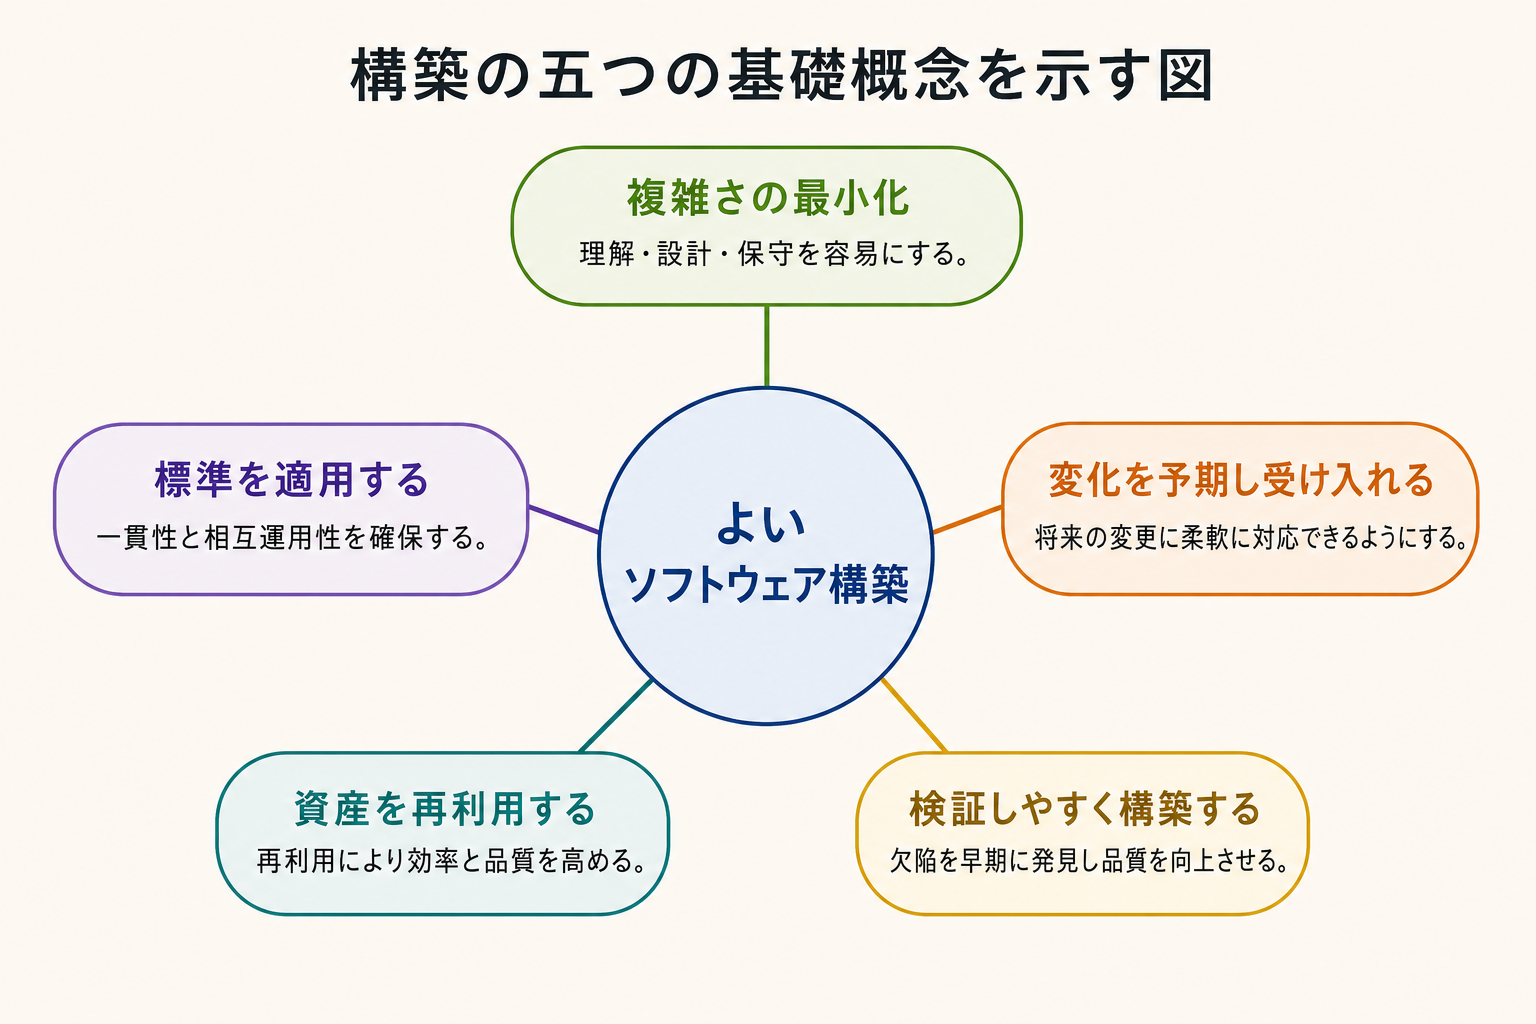
\includegraphics[width=0.96\linewidth]{assets/generated_figures/ch04/fig-ch04-03.png}}{\fbox{\parbox[c][48mm][c]{0.9\linewidth}{\centering 画像生成待ち\\構築の五つの基礎概念を示す図}}}
\caption{構築の五つの基礎概念を示す図}
\label{fig:ch04-03}
\end{figure}
